\documentclass[a4paper,10pt]{article}
%\documentclass[preview=false]{standalone}
% %%%% Define new conditional \ifplastex
% %%%% This ensure that the file complied normally without plasTeX.
\usepackage{plastex}

\ifplastex\else
\usepackage{standalone} %%%% Only load standalone when not in plasTeX
\standalonetrue
\fi

% % Package for typesetting URLs
\usepackage{url}

\usepackage{import}

\usepackage{iumlb}

\usepackage{multirow}

% Package for including figures
\usepackage{graphicx}

% Package for sub-floats (e.g. figures)
\usepackage{subfig}

% % Title
\title{iUML-B Class Diagrams User Manual} 

% % Author
\author{Colin Snook\\University of Southampton}

% % Date
\date{%
	Version 0.0.1\\%
	\today%
}

\begin{document}
	\ifplastex%
	\maketitle% Make title if in plasTeX mode.
	\else%
	\ifstandalone%
	\maketitle % Make title if in standalone mode.
	\else%
	\fi%
	\fi%
	
	This section will cover iUML-B Class diagrams.
	
	
	\section{Class Attributes}
\label{sec:classdiagrams-attributes}



\paragraph{Initial Value } 
The initial value field is a Rodin Keyboard text field. 
The string in the text field is used as the intialisation value for the owning class attribute (or association) but can be interreted in several ways:
\begin{itemize}
	\item If the attribute is owned by a variable instance class, this field is currently ignored. (It should be used in a constructor).
	\item If the attribute elaborates a constant, this field is ignored. 
	\item If the attribute elaborates a variable, an action is added to the Initialisation event to intialise the attribute. as follows:
	\begin{itemize}
		\item if the text field begins with one of the Event-B assignment operators it is used to assign to the complete attribute relation (i.e. expression = attribute.name+initialValue.String)
		\item otherwise the text is assumed to contain the value to be assigned to each and every instance \\(i.e. expression = attribute.name+":="+class.name+"X"+initialValue.String)
	\end{itemize}	
\end{itemize}


%%% Local Variables:
%%% mode: latex
%%% TeX-master: "iuml-b-classdiagrams-user_manual"
%%% End:

	%
	%\section{Getting Started}
\label{sec:iumlb-gettingstarted}

Since iUML-B diagrams are contained within Event-B machines, start by creating an Event-B project containing a Machine project. 
Then select the machine in the Event-B navigator and right click to use the context manual. 
The context manual contains commands to add the various kinds of iUML-B diagram to the machine.

Once the machine contains a diagram, it will appear in the Event-B navigator as an element within the machine.
To open the diagram for editing, double click on the iUML-B element in the Event-B navigator.

You can now use the diagram editor palette to create new elements on the canvas. 
Use the properties sheet to edit the detailed properties of an element.
Refer to the diagram specific user manuals within this manual.

Once the diagram model has been entered, the toolbar buttons can be used to process it.
The validate button (tick icon) runs a diagram validation test to check that the diagram is well-formed.
This validation is also performed automatically before you generate from the diagram.
To generate Event-B use the translate button (UML-B icon). 
The rules for generation of Event-B are given in the diagram specific manuals.

There is also a command (`Translate All iUML-B Diagrams') in the context manual of the machine (right click the machine in the Event-B navigator).
This translates all of the iUML-B diagrams contained in the machine.

\begin{figure}[!htbp]
	\centering
	\ifplastex
	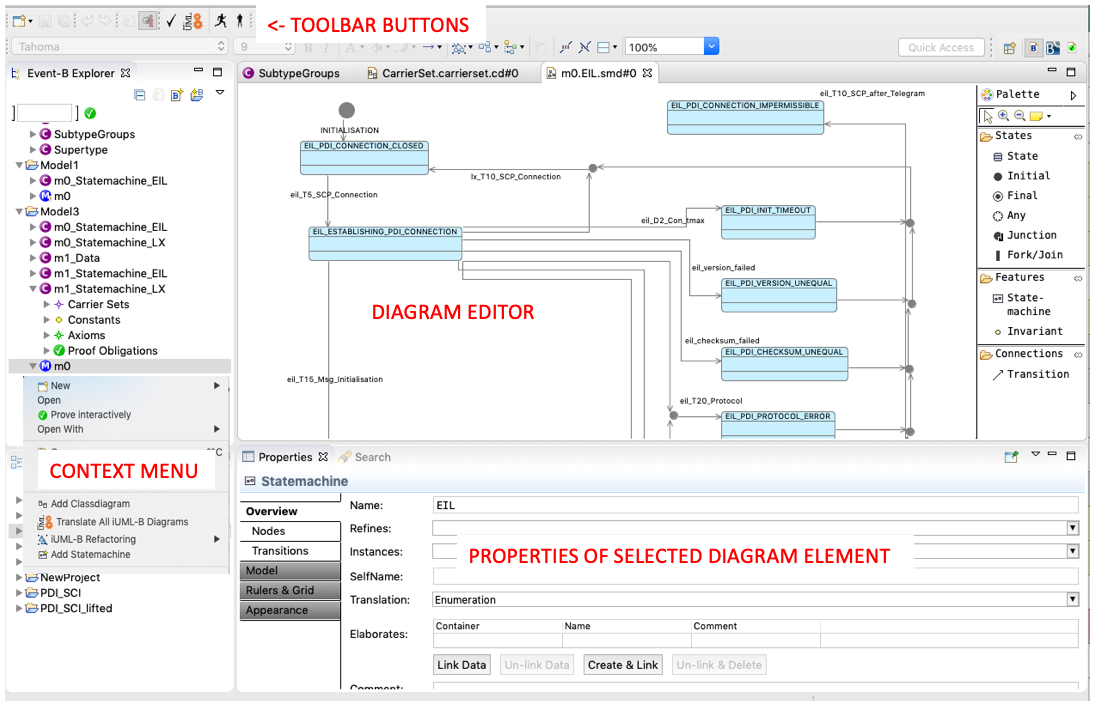
\includegraphics[width=1000]{figures/UMLB_UI.png}
	\else
	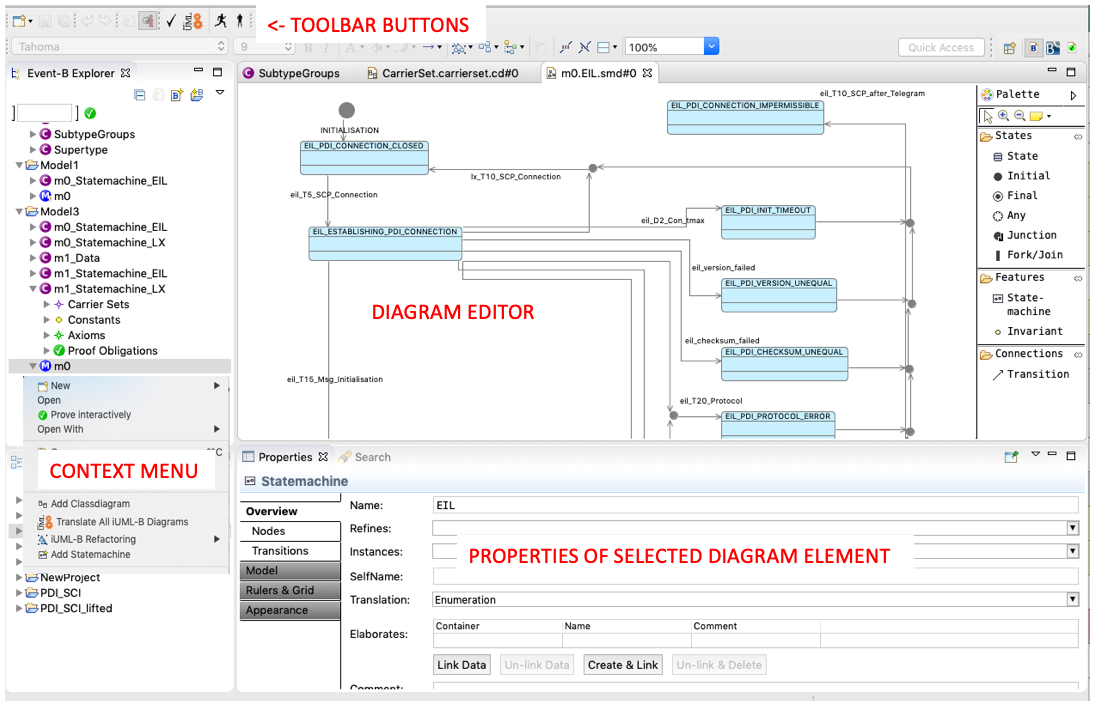
\includegraphics[width=1\textwidth]{figures/UMLB_UI.png}
	\fi
	\caption{User Interface for iUML-B}
	\label{fig:UMLB_UI}
\end{figure}
	%
	%\section{Concepts}
\label{sec:iumlb-concepts}

The iUML-B diagrams generate Event-B which is annotated as generated.
The generated Event-B is read-only and editors (should) not allow you to edit it.
You can however, add manually entered elements to the Event-B machine alongside the generated ones.
The intention is to allow users both options: modelling by diagram, modelling in Event-B.

As well as generating new Event-B elements, iUML-B often \emph{elaborates} existing Event-B elements.
In the latter case, the iUML-B model element contributes to the definition or children of the elaborated element.
For example, an invariant could be generated to constrain the elaborated element.


	%
	%\input{iuml-b-tasks}
	%
	%\input{iuml-b-reference}
	%
	%\section{Refactoring}
\label{sec:component_diagrams-refactoring}

A refactoring facility is provided in iUML-B that allows a set of changes made to the collection of iUML-B diagrams in an abstract model to be propagated down the refinement chain as part of a commit action. Alternatively, the set of changes can be reverted, restoring the model to its pre-change state.
Changes cannot be committed (hence propagated) when a lower refinement also has uncommitted changes. I.e. if several refinements have uncommitted changes they must be committed or reverted in order starting from the most refined level and working up the refinement chain. 
Changes are only propagated to a refinement when they are still relevant to the refinement. Changes may have already been made in the refinement, as part of the refinement process, that mean that a subsequent change in the abstract model cannot be propagated. For example the parent element of a changed attribute may have been removed and replaced with a different model element or a guards predicate may have been edited to utilise new variables introduced in the refinement. Changes to Event-B formula attributes (i.e. predicates and actions) are only propagated when the equivalent refined formula is unchanged except for formatting (whitespace).

\subsection{Enabling Refactoring}

The refactoring facility may be enabled or disabled in the iUML-B preferences menu (Figure \ref{fig:PreferenceForEnablingRefactoring}). The current default is DISABLED.  
WARNING: If this preference is disabled while there are outstanding, uncommitted changes, and the associated model is then edited without refactoring being enabled, those change records will become invalid and wont be able to be propagated at a later stage.

 \begin{figure}[!htbp]
  \centering
  \ifplastex
  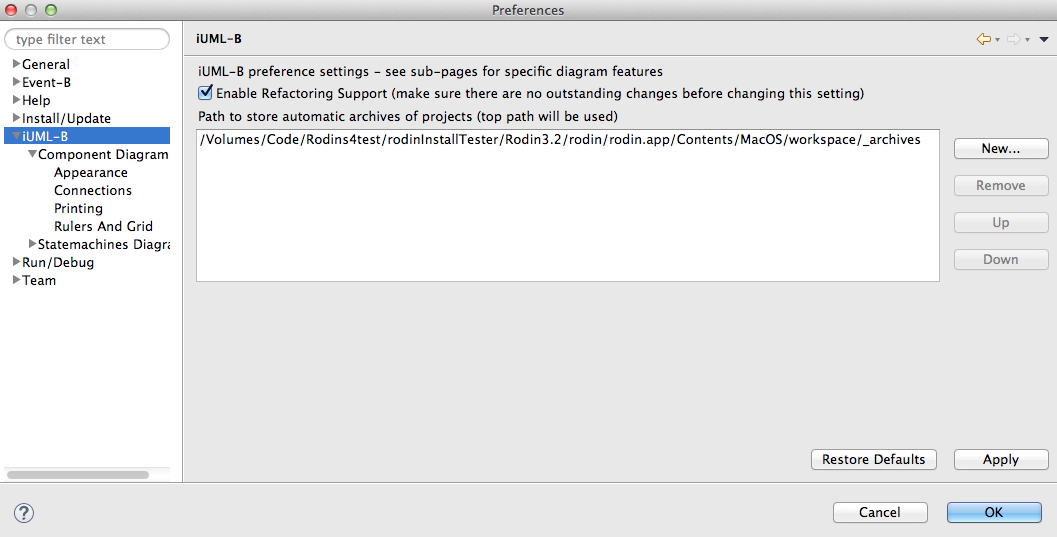
\includegraphics[width=1024]{figures/image59.png}
  \else
  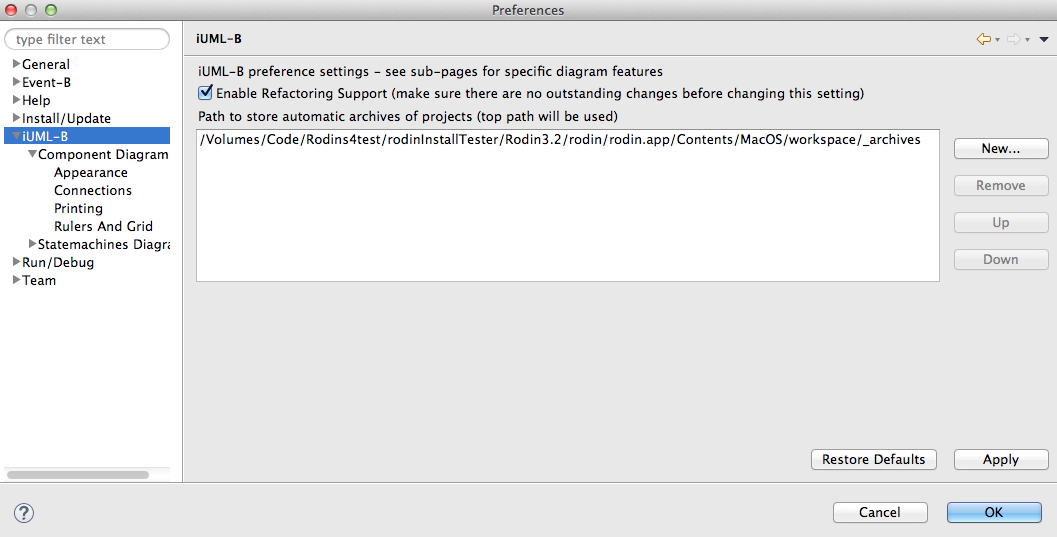
\includegraphics[width=1\textwidth]{figures/image59.png}
  \fi
  \caption{Preference for Enabling Refactoring}
  \label{fig:PreferenceForEnablingRefactoring}
\end{figure} 

\subsection{Automatic Archiving}

An archive of the complete project including any change records and reports is made before a commit is attempted. This is in case an unexpected event such as power failure should cause the commit to fail leaving the model in a corrupted state. In this case the project should be deleted and restored from the archive using the standard Eclipse import facility (\textbf{\texttt{Import - General - Existing Projects into Workspace - Select archive file}}).

\subsection{Decorator}

Machines with outstanding, uncommitted changes are decorated in the Event-B Explorer (Figure \ref{fig:DecoratorIndicatingOutstandingRecordedChanges}). 

 \begin{figure}[!htbp]
  \centering
  \ifplastex
  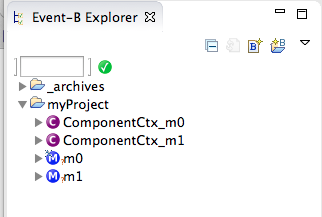
\includegraphics[width=1024]{figures/image60.png}
  \else
  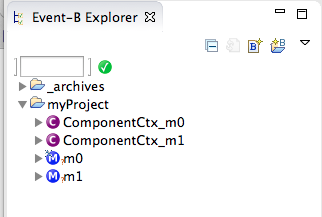
\includegraphics[width=1\textwidth]{figures/image60.png}
  \fi
  \caption{Decorator Indicating Outstanding Recorded Changes (see M0)}
  \label{fig:DecoratorIndicatingOutstandingRecordedChanges}
\end{figure} 

\subsection{Refactoring Menu: Commit and Revert}

The Commit and Revert actions are accessed from a pop-up context menu, by right clicking on a machine that has outstanding uncommitted changes (Figure \ref{fig:ContextMenuForCommitRevert}).

 \begin{figure}[!htbp]
  \centering
  \ifplastex
  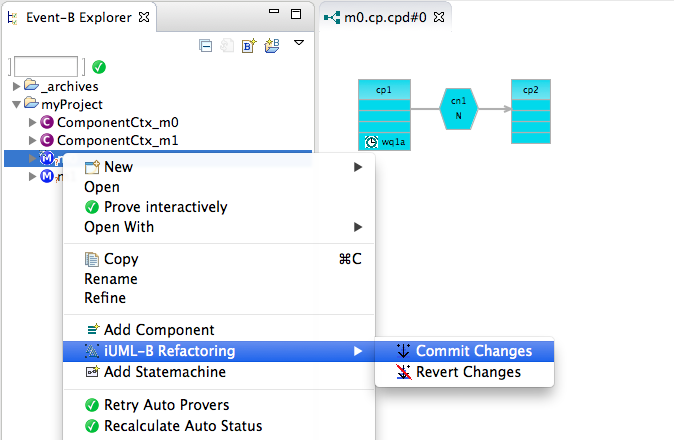
\includegraphics[width=1024]{figures/image61.png}
  \else
  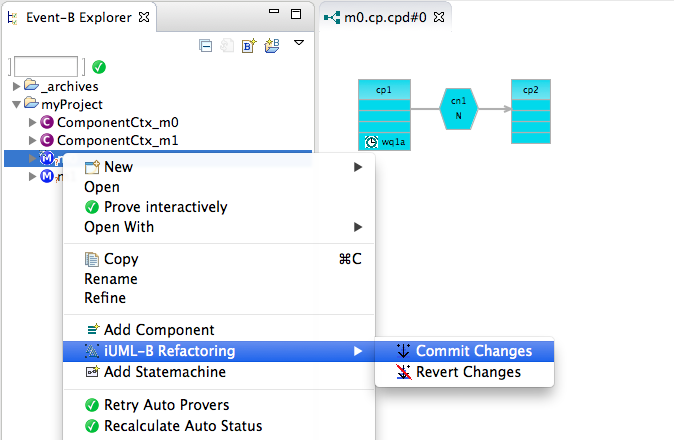
\includegraphics[width=1\textwidth]{figures/image61.png}
  \fi
  \caption{Context Menu for Commit/Revert}
  \label{fig:ContextMenuForCommitRevert}
\end{figure} 

\textbf{Commit} -
When Commit is selected for a machine that has outstanding uncommitted changes, firstly an information and confirmation message appears (Figure \ref{fig:CommitConfirmationMessage}). This gives the user a chance to cancel since the Commit operation is a significant process that can only be reversed by restoring from archive.

 \begin{figure}[!htbp]
  \centering
  \ifplastex
  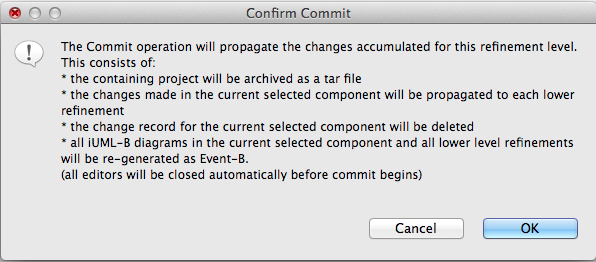
\includegraphics[width=1024]{figures/image62.png}
  \else
  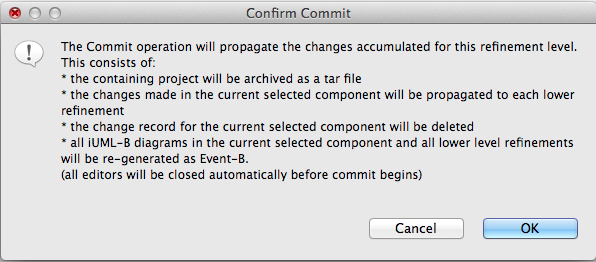
\includegraphics[width=1\textwidth]{figures/image62.png}
  \fi
  \caption{Commit Confirmation Message}
  \label{fig:CommitConfirmationMessage}
\end{figure} 

If ok is selected on Mi, the following steps will be taken
\begin{enumerate}
\item any open diagrams will be closed, 
\item the project will be archived,
\item the recorded changes for Mi will be propagated to the next level refinement Mi+1 (if any),
\item the changes made to the refinement Mi+1 will be recorded,
\item the previous change records for Mi will be deleted,
\item all diagrams of the previous model Mi will be generated,
\item steps 3 to 6 will be repeated for the refinement Mi+1,
\item a report of the complete process will be saved.
\end{enumerate}


\textbf{Revert} -
When Revert is selected for a machine that has outstanding uncommitted changes, firstly an information message appears (Figure \ref{fig:RevertConfirmationMessage}). This gives the user a chance to cancel since the Revert operation is a significant process that cannot be reversed.

 \begin{figure}[!htbp]
  \centering
  \ifplastex
  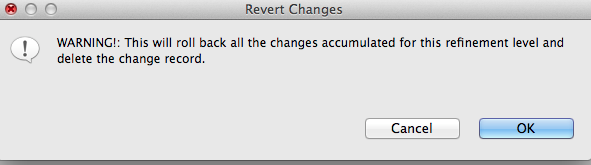
\includegraphics[width=1024]{figures/image63.png}
  \else
  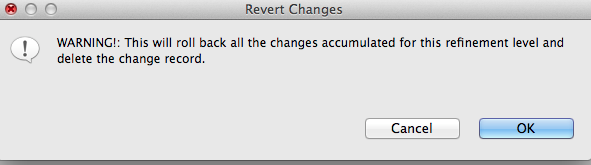
\includegraphics[width=1\textwidth]{figures/image63.png}
  \fi
  \caption{Revert Confirmation Message}
  \label{fig:RevertConfirmationMessage}
\end{figure} 

If ok is selected on a machine Mi, the following steps will be taken
\begin{enumerate}
\item any open diagrams will be closed,
\item the changes made to Mi will be reverted taking the model back to its original state,
\item the change records for Mi will be deleted,
\item all diagrams of Mi will be generated.
\end{enumerate}


\textbf{No Changes} - 
If Commit or Revert are selected for a machine that has no recorded changes, an appropriate message is displayed (Figure \ref{No Changes Error Message})and no further action is taken.

 \begin{figure}[!htbp]
  \centering
  \ifplastex
  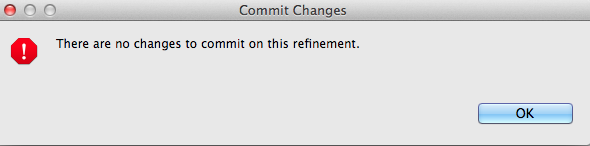
\includegraphics[width=1024]{figures/image64.png}
  \else
  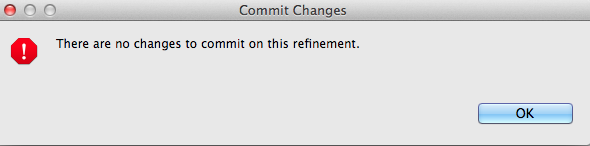
\includegraphics[width=1\textwidth]{figures/image64.png}
  \fi
  \caption{No Changes Error Message}
  \label{fig:NoChangesErrorMessage}
\end{figure} 

\subsection{Resources: Change Records and Reporting}

Various resources are created to support refactoring. In normal use it is not necessary to access these resources and they are not visible in the Event-B Explorer by default. If it is wished to examine the generated reports or the change records they can be viewed either by opening a standard Eclipse workspace file navigator or Project Explorer (using Window-Show View) or by un-selecting the All files and folders filter of the Event-B Explorer. (The second method is shown in Figure \ref{fig:RemovingAllFilesAndFoldersFilterForEventBExplorer}).

 \begin{figure}[!htbp]
  \centering
  \ifplastex
  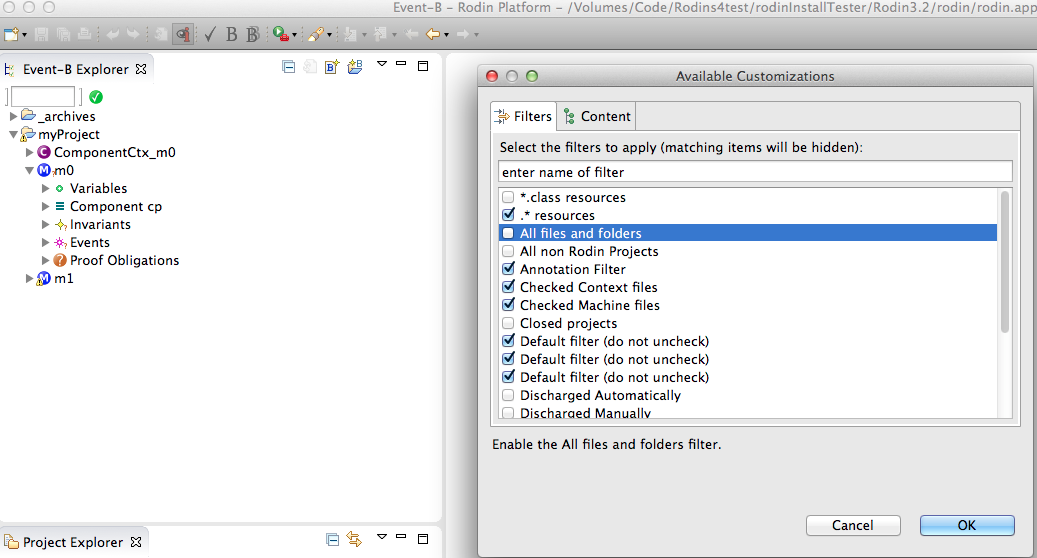
\includegraphics[width=1024]{figures/image65.png}
  \else
  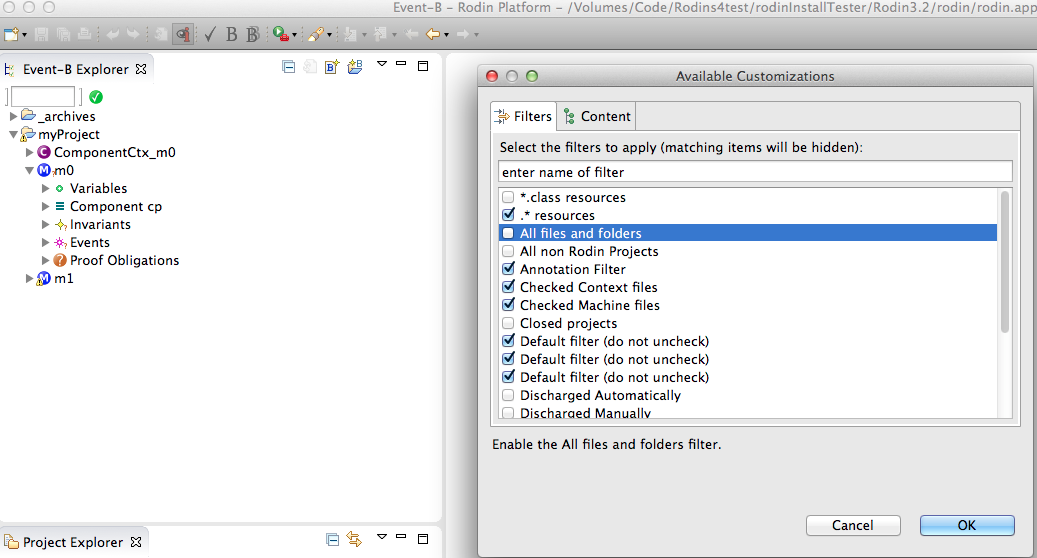
\includegraphics[width=1\textwidth]{figures/image65.png}
  \fi
  \caption{Removing `All files and folders' Filter for Event-B Explorer}
  \label{fig:RemovingAllFilesAndFoldersFilterForEventBExplorer}
\end{figure} 

The various resources that are generated (Figure \ref{fig:ChangesResourcesProducedForRefactoring}) are as follows. 
As soon as a supported editor is opened two files will appear in a folder called /iumlb/changes/ within the project. These are:
$<$myMachine$>$\_bum.xmb  -  a copy of the pre-change state of the model,
$<$myMachine$>$\_bum.equivmap - a map from the elements in the xmb file to the corresponding elements in the Rodin  model. 
These files can be opened for examination but if they are edited the refactoring process is likely to fail. The xmb file can be opened with an EMF editor such as Rose. The equivmap file can be opened with a normal text editor.
As soon as some changes to the diagram are saved a change record will appear in the same folder, $<$myMachine$>$\_bum.changes.  Again, the file can be opened with an EMF editor such as Rose but any alterations are likely to cause the refactoring process to fail.

 \begin{figure}[!htbp]
  \centering
  \ifplastex
  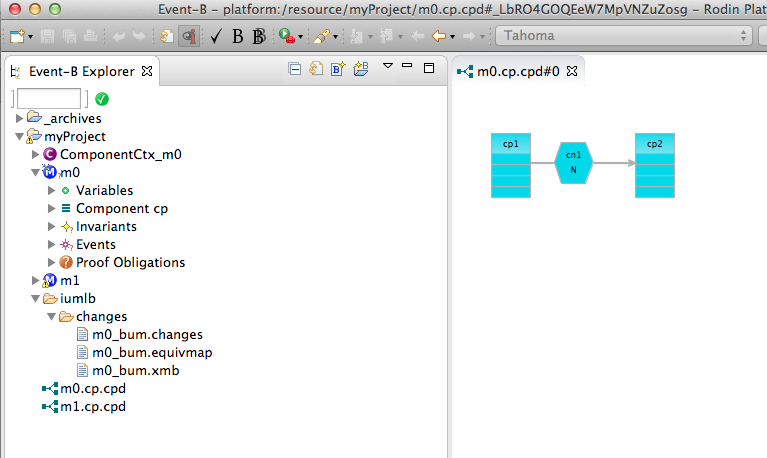
\includegraphics[width=1024]{figures/image66.png}
  \else
  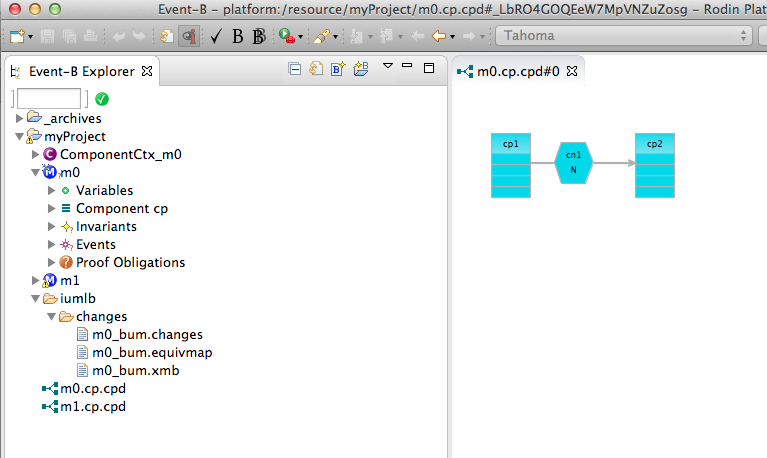
\includegraphics[width=1\textwidth]{figures/image66.png}
  \fi
  \caption{Changes Resources Produced for Refactoring}
  \label{fig:ChangesResourcesProducedForRefactoring}
\end{figure} 

Note: If these three files are deleted the project will be left in its current state with no record of changes. This can be useful if for some reason it is wished to neither commit nor revert the changes but to leave the models as they are with the abstract model edited but the changes not propagated. 
If the changes are reverted, once the revert process has completed, these three files are deleted.
If the changes are committed, once the commit has completed, these three files are deleted and a file $<$myMachine$>$\_bum.$<$timestamp$>$.report is created in the folder /iumlb/reports/. This is a text file giving a detailed record of the changes made down the refinement chain (Figure \ref{fig:ReportsProducedByRefactoring}).

 \begin{figure}[!htbp]
  \centering
  \ifplastex
  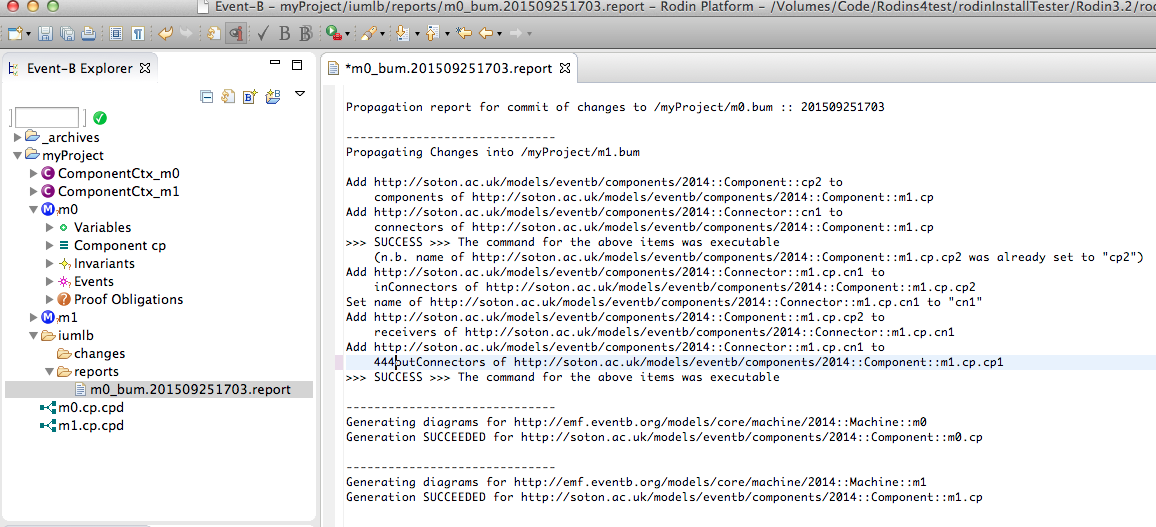
\includegraphics[width=1024]{figures/image67.png}
  \else
  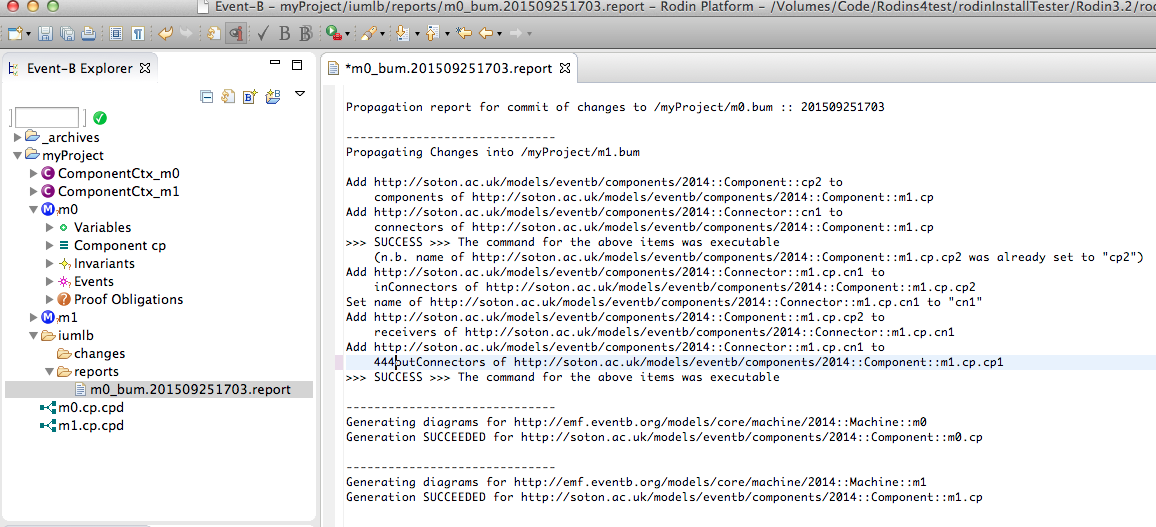
\includegraphics[width=1\textwidth]{figures/image67.png}
  \fi
  \caption{Reports Produced by Refactoring}
  \label{fig:ReportsProducedByRefactoring}
\end{figure} 

%%% Local Variables:
%%% mode: latex
%%% TeX-master: "component_diagrams-user_manual"
%%% End:

	
\end{document}

%%% Local Variables:
%%% mode: latex
%%% TeX-master: t
%%% End: